\newpage
\thispagestyle{empty}
\mbox{}

\ifdefined\included
\else
\setcounter{chapter}{2} %% Numéro du chapitre précédent ;)
\dominitoc
\faketableofcontents
\fi

\chapter{Models and Algorithms to Integrate Theory of Mind in Human-Aware Task Planning}
\chaptermark{Models and Algorithms of Theory of Mind}
\label{chap:3}
\minitoc

\chapabstract{This chapter presents my first main contribution, proposing models and algorithms to incorporate Theory of Mind concepts in \acrshort{hrc} task-planning. An empirical evaluation is provided and discussed, demonstrating how this contribution solves a broader class of problems than HATP/EHDA, without systematically using communication.}

%%% SECTION %%%%%%%%%%%%%%%%%%%%%%%%%%%%%%%%%%%%%%%%%%%%%%%%%%%%
\section{Introduction}

\begin{figure}[h]
    \centering
    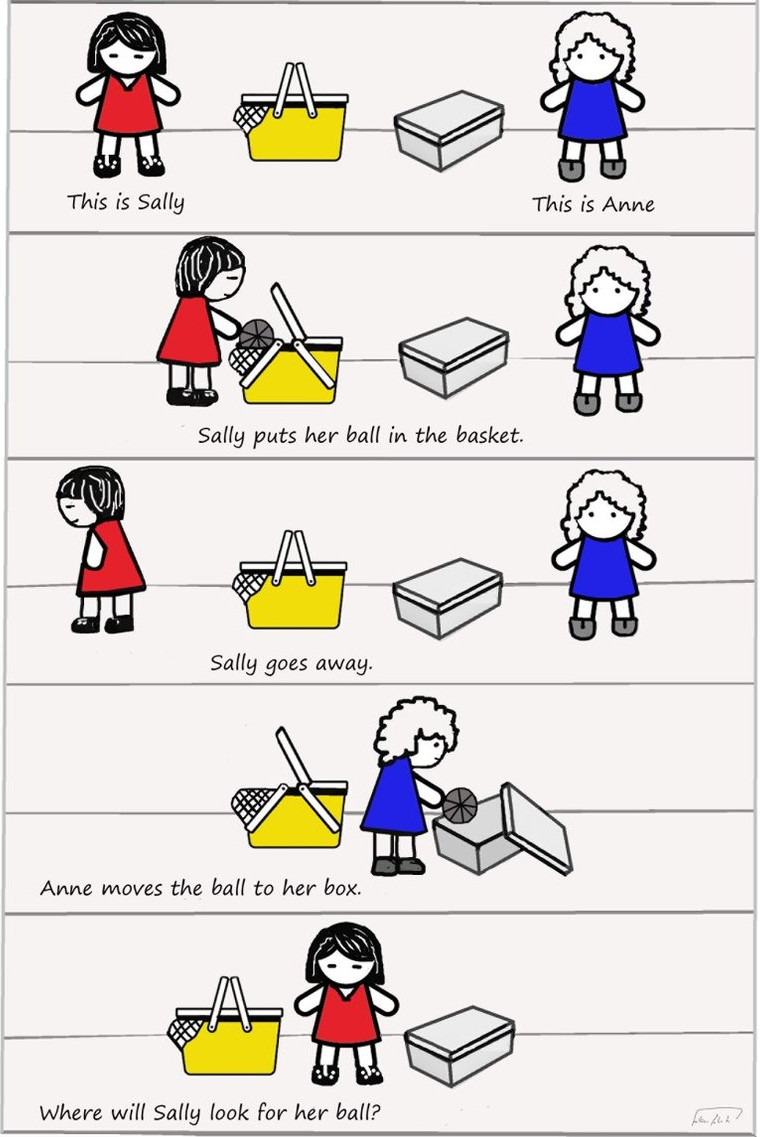
\includegraphics[width=0.5\linewidth]{Chapter3/The-Sally-Anne-Task.jpeg}
    \caption{Sally and Anne Task}
    \label{fig:sally_and_anne_task}
\end{figure}

False belief tasks are commonly used as tests to acknowledge the presence of Theory of Mind reasoning. The most common test is the \textit{Sally and Anne} one, depicted in fig~\ref{fig:sally_and_anne_task}. It is used in developmental psychology to examine children's ``theory of mind'' understanding, which refers to their ability to understand how other people think, feel and behave. The test consists of describing the execution of a simple task involving non-observable facts and co-presence. Then, children are questioned about the beliefs of one of the characters. The task consists of the following. Sally and Anne are two co-present characters near a basket and a box. Sally puts her ball in the basket before going away. Then, in hindsight, Anne moves the ball from the basket to the box. Finally, Sally comes back to look for her ball. The following question is now asked: ``Where will Sally look for her ball?''. As an observer of this scene, using Theory of Mind, we can naturally say that Sally will look for her ball in the basket because this is where she left it, and she is unaware of Anne's action. Young children cannot understand that Sally has different beliefs from theirs and, thus, they are likely to answer that Sally will look in the box. 

\acrfull{tom} reasoning is critical for interaction and collaboration between agents. Thus, it is reasonable and desirable to endow robots with such skills to enhance their interactions with humans. This is the motivation of the contribution presented in this chapter. We propose an extension of HATP/EHDA to maintain human beliefs during the planning process in a principled way in order to anticipate and tackle estimated false human beliefs that may be detrimental to task resolution.

Some works consider \acrshort{tom} during execution to handle unexpected situations and contingencies like \cite{devin_implemented_2016}. 
However, such reactive approaches are not always enough since deadends can require proactive decisions and actions to be avoided. 

We would want the robot to be able to reason and correctly maintain distinct human beliefs. Despite HATP/EHDA modeling distinct beliefs, this scheme does not maintain them automatically. The beliefs can only be updated in a scripted way through the description of action effects provided in the planning problem. We propose models and algorithms to integrate concepts of the Theory of Mind in the planning process of HATP/EHDA. This way, the robot can accurately estimate human beliefs and better predict their behavior. Moreover, we propose solutions for the robot when tackling estimated false human beliefs that may impact the task resolution.


%%% SECTION %%%%%%%%%%%%%%%%%%%%%%%%%%%%%%%%%%%%%%%%%%%%%%%%%%%%
\section{Related work}

    This chapter's contribution is related to several topics that have not been mentioned yet. Hence, this section introduces the new topics and relevant related work to capture our contribution better.  

    \subsection{Theory of Mind in HRC}
    \acrfull{tom} refers to the ability to attribute mental states to oneself and others, such as beliefs, desires, and intentions. However, estimating the current knowledge and beliefs of the different agents is challenging. To do so, we must consider Theory of Mind concepts, especially perspective shift and the notion of co-presence.
    
    Robots endowed with \acrshort{tom} abilities are more effective in proactive robotic assistance and are perceived as more socially intelligent by humans \cite{shvo_proactive_2022}. \acrshort{tom} enables robots to infer human desires, beliefs, and intentions, allowing for natural interaction between robots and humans \cite{yu_robot_2023}. Robots with \acrshort{tom} can anticipate human strategies and incorporate them into their decision models, leading to better team performance \cite{romeo_exploring_2022}. The presence of \acrshort{tom} in robots influences human decision-making behavior and trust, making it more appropriate for human-robot collaboration \cite{schlobach_abstracting_2022}. Computational theory of mind, based on abstractions of beliefs into higher-level concepts, facilitates collaboration on decisions and improves the quality of human decisions \cite{gurney_robots_2022}. However, the lack of a unified construct and consistent benchmarking hinders progress in endowing robots with \acrshort{tom} capabilities.

    In \cite{devin_implemented_2016}, Theory of Mind improves shared plan execution. 
    Humans' temporary absence or inattention during collaboration can induce insufficient knowledge about the current situation. The robot might need to detect such situations and be able to provide the information about the missing or incorrect information to its human partner without being annoying or intrusive. To do so, they propose a framework that allows the robot to estimate the other agents' mental states about the environment and the state of goals, plans, and actions. 
    In \cite{lemaignan_underworlds_2018}, the proposed framework named UNDERWORLDS allows cascading situation assessment to estimate other agents' beliefs during execution. The two previous frameworks can estimate and track the human partner's belief in order to reactively adapt the robot's actions during execution. However, they are not designed to be used during task planning to make proactive robot actions to avoid a potential false belief.


    %%% SUB-SECTION %%%%%%%%%%%%%%%%%%%%%%%%%%%%%%%%%%%%%%%%%%%%
    \subsection{Epistemic Planning}
    Epistemic planning helps to plan the correct sequence of actions to reach a desired knowledge, including a desired world state. Thomas Bolander is one of this field's main contributors and describes it as follows in \cite{bolander_gentle_2017}. Epistemic Planning is the enrichment of planning with epistemic notions, that is, knowledge and beliefs. The human or robot might have to reason about epistemic aspects such as: Do I know at which post office the parcel is? If not, who would be relevant to ask? Maybe the parcel is a birthday present for my daughter, and I want to ensure that she does not get to know about it, and I have to plan my actions accordingly (make sure she does not see me with the parcel). The epistemic notions are usually formalized using epistemic logic. Epistemic planning can naturally be seen as combining automated planning with epistemic logic, relying on ideas, concepts, and solutions from both areas. 

    It enables robots to make plans to achieve the required knowledge and to reason about the knowledge and capabilities of other agents, ensuring effective collaboration and coordination in human-robot interactions \cite{belle_epistemic_2023}.

    Bolander et al. proposed the \acrfull{del} approach \cite{bolander_gentle_2017} and even implemented some Theory of Mind concepts in it. However, despite being more expressive than HATP/EHDA, this approach does not maintain human beliefs in a principled way either. They tend to use domain-specific rules given in the problem specification, usually with conditional action effects. 

    Muise et al. worked on multi-agent epistemic planning using a classical planning approach~\cite{muise_planning_2015}. Since involving nested beliefs is computationally demanding, their work proposes to convert and encode such problems into classical planning problems. Hence, state-of-the-art classical planning techniques can tackle nested beliefs of multiple agent problems. 

    
    \subsection{Communication in HRC}

    Communication enables effective interaction between humans and robots, promoting inclusivity and reducing obstacles in human-robot interaction. Communication allows robots to share information about their actions and intentions, enhancing transparency and explainability \cite{mcmillan_human-robot_2023}. It helps establish trust and understanding between humans and robots, leading to improved teamwork and performance \cite{verhagen_influence_2022}. 
    Adapting conversational strategies to optimize performances and engagement is also important and addressed in \cite{galland_adapting_2022}.
    Non-verbal gestures and behavior of robots during collaboration can impact the robot's perception and influence the willingness of humans to cooperate \cite{arntz_collaborating_2022}. Communication also allows robots to assess their own skills and limitations, propose alternatives, and adapt the execution of tasks to the capabilities of the collaborators \cite{ferrari_bidirectional_2022}. Overall, effective communication facilitates mutual knowledge, enables the exchange of information, and allows humans and robots to work together efficiently and successfully.


%%% SECTION %%%%%%%%%%%%%%%%%%%%%%%%%%%%%%%%%%%%%%%%%%%%%%%%%%%%
\section{Maintaining the Human Beliefs while Planning}

    %%% SUB-SECTION %%%%%%%%%%%%%%%%%%%%%%%%%%%%%%%%%%%%%%%%%%%%
    \subsection{Enhanced Problem Specification}

As an example and for illustration purposes, let us consider cooking pasta as a human-robot collaborative shared task. This scenario is depicted in figure~\ref{fig:cooking_task}.

\begin{figure}[h]
    \centering
    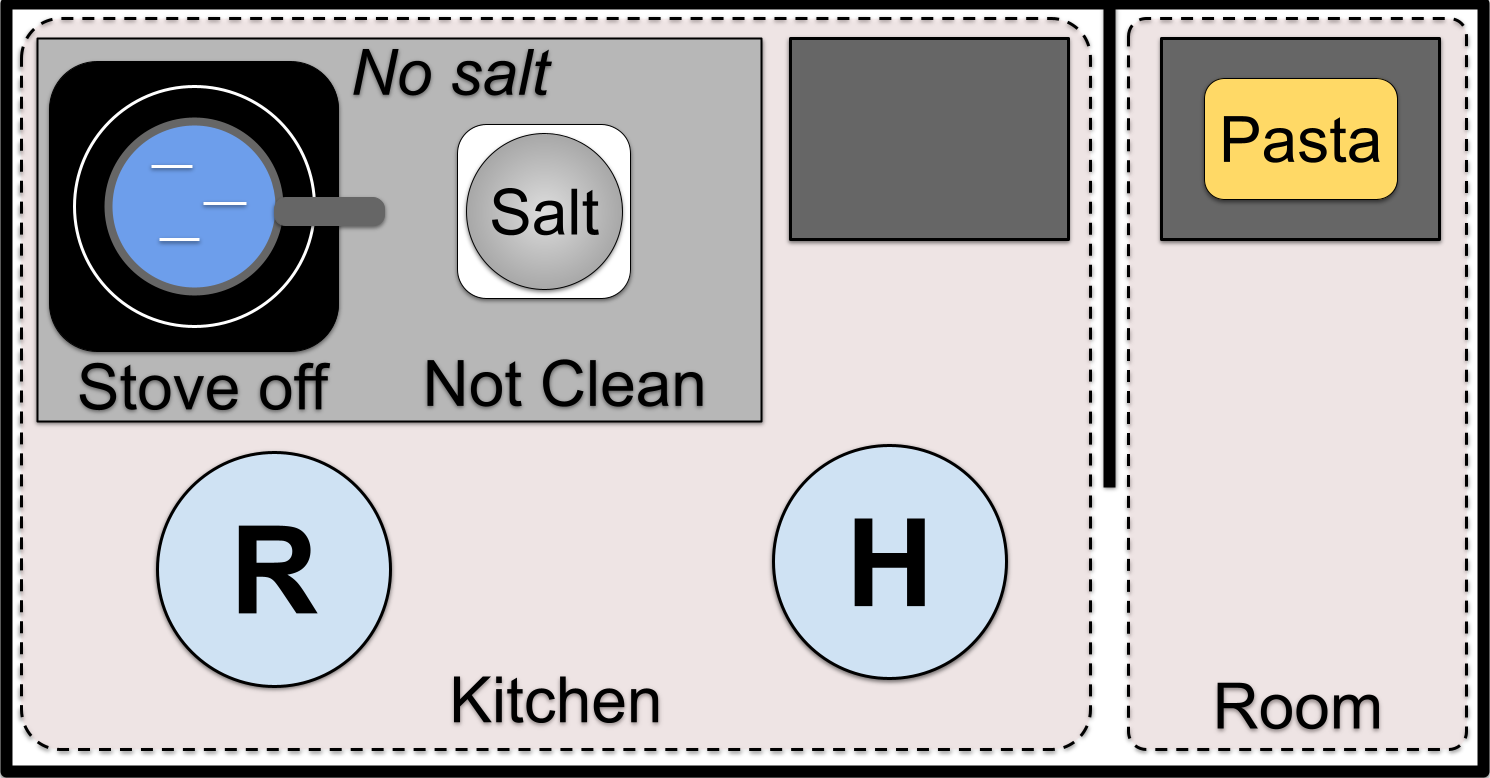
\includegraphics[width=0.6\linewidth]{Chapter3/cooking_task_draw.png}
    \caption{
        A cooking pasta collaborative shared task. It consists of turning on the \textit{stove}, adding \textit{salt} in the pot, \textit{fetching} the pasta, and \textit{pour} the pasta in the pot. Additionally, the robot has to \textit{clean} the counter. However, there are two seperated rooms and both the presence of salt in the pot and the clean aspect of the counter are not observable facts, possibly causing false beliefs.
    }
    \label{fig:cooking_task}
\end{figure}

The robot has to turn on the stove (\textit{stoveOn}) and clean the counter (\textit{counterClean}), but the latter is not a part of the shared task. The human takes care of fetching the pasta while both agents can add salt into the water (\textit{saltIn}). Before pouring the pasta into the pot, the human must know the facts, \textit{stoveOn} and \textit{saltIn}. 
Unlike \textit{stoveOn}, the facts \textit{saltIn} and \textit{counterClean} are not directly observable. 
Hence, by acting while the human is away fetching the pasta, the robot may induce false beliefs, which may be detrimental to the shared task (\textit{e.g.}, the human adding salt again).

To describe this problem we start from the HATP/EHDA problem specification, which is the one described in Chapter~\ref{chap:2}. For our collaborative cooking example, the sets $B$ and $X$ for the collaborative cooking example are the following:
{\small
\begin{align*}
&B           = Entities \cup Places \cup Booleans \cup \{\textsf{nil}\} \\
&\quad Entities    = Agents \cup Objects\\
&\quad Agents      = \{ \textsf{R}, \textsf{H} \} ~~ \backslash\backslash~\textsf{R}:robot,~\textsf{H}:human\\
&\quad Objects     = \{ \textsf{salt}, \textsf{pasta}, \textsf{counter} \}\\
&\quad Places      = \{ \textsf{kitchen}, \textsf{room} \}\\
&\quad Booleans    = \{ \textsf{true},\textsf{false} \}\\
&\\
&X = \{ at(e)~|~ e \in Entities, ~saltIn, ~stoveOn, ~counterClean  \}\\
&\quad \textit{Range}(saltIn ~|~ stoveOn ~|~ counterClean)=Booleans\\
&\quad \textit{Range}(at(\textsf{R} ~|~ \textsf{H} ~|~ \textsf{pasta})) = Places\\
&\quad \textit{Range}(at(\textsf{salt} ~|~ \textsf{counter})) = \{ \textsf{kitchen} \}
\end{align*}
}

Our first contribution starts from here, where we augmented the specification by associating each state-variable $x_i \in X$ to a location and an observability type. Thus, we define two other functions besides the \textit{variable value assignment} function (Definition~\ref{def:variable_value_assignment_function}) to assign observability types (Definition~\ref{def:variable_observability_assignment_function}) and locations (Definition~\ref{def:variable_location_assignment_function}) to state-variables.

\begin{definition}
    \textbf{(Variable observability assignment function $obs$.)} A \emph{variable observability assignment function} over $X$ is a function $\obsf$ that maps each $x_k \in X$ into an observability type $t_j \in \{ \texttt{OBS},  \texttt{INF} \}$, s.t., $\obsf = \{ (x_1,t_1), \ldots , (x_n,t_n) \}$. With $\obsf(x_k) = \texttt{OBS} | \texttt{INF}$, $x_k$ is said to be respectively \textit{observable} $|$ \textit{inferable}.
    We use the following notation to access the observability type $t_j$ of the state-variable $x_k$ in the state $s_i$: $\obsf[i](x_k) = t_j$.
    \label{def:variable_observability_assignment_function}
\end{definition}

\begin{definition}
    \textbf{(Variable location assignment function $loc$.)} A \emph{variable location assignment function} over $X$ is a function $\locf$ that maps each $x_k \in X$ into a $l_j \in Places \cup \{ \texttt{nil} \}$, s.t., $\locf = \{ (x_1,l_1), ..., (x_n,l_n) \}$. 
    $Places \subseteq B$ captures a group of constant symbols such that each member is a predefined area in the environment. 
    Agents are always either ``situated'' in a place or moving between two places. 
    We consider $x_i$ to be located in every $place \in Places$ if $\locf(x_i)=\texttt{nil}$. 
    We use the following notation to access the location $l_j$ of a state-variable $x_k$ in the state $s_i$: $\locf[i](x_k) = l_j$.
    \label{def:variable_location_assignment_function}
\end{definition}

% Then, a \textit{variable location assignment} function over $X$ is a function $\locf$ that maps each $x_i \in X$ into a $l_i \in Places \cup \{ \texttt{nil} \}$: $\locf = \{ (x_1,l_1), ..., (x_n,l_n) \}$. 
% $Places \subseteq B$ captures a group of constant symbols such that each member is a predefined area in the environment. 
% Agents are always either ``situated'' in a place or moving between two places. 
% We consider $x_i$ to be located in every $place \in Places$ if $\locf(x_i)=\texttt{nil}$. 
% When discussing the beliefs updates, more details about how the environment should be divided into places will be given shortly.

The observability and location of the state-variable are internal to the robot but assumed to be common to both agents. Consequently, we update our \textit{state} definition (def.~\ref{def:state}) to take them into account in the new definition~\ref{def:state_tom}.

\begin{definition}
    \textbf{(State $s$.)} In this contribution, in addition to both agent states, a \emph{state} now comprises the two novel assignment functions $\obsf$ and $\locf$, s.t., $s_i = \{ \agentstate[R][i], \agentstate[H][i], \obsf[i], \locf[i] \}$.
    \label{def:state_tom}
\end{definition}

This new definition still consider the two agent states s.t. $\agentstate[\agent][i] = \{ \valf[\agent][i], \agenda[\agent][i], \partialplan[\agent][i] \}$. Now, in each state, we keep track of each state-variable's observability type and location, and we can reason on them to update the human beliefs ($\valf[H]$) accordingly. 

We remind definition~\ref{def:false_belief} stating that a state $s_i \in S$ contains \textbf{false beliefs}, or \textbf{belief divergences}, if $\exists x_j \in X, \valf[H][i](x_j) \neq \valf[R][i](x_j)$. That is, if any state-variable has a different value in the human beliefs \textit{w.r.t.} the robot one, we assume the human has a false belief about those particular state-variables. Since the planner is part of the robot, we assume the robot beliefs are true and correspond to the ground truth. Consequently, any divergence between the two beliefs is assumed to be a human false belief, as it would make no sense to keep false information in the robot's beliefs. 

The initial state of our cooking example can be described as follows. There is no initial belief divergence, the initial partial plans are empty, and both agents perform the shared cooking task named $CookPasta$. In addition, the robot must clean the kitchen counter once the cooking is done. Hence, the task $CleanCounter$ is added to the initial robot agenda after the shared task. The only \textit{non-obversable} facts are the presence of salt in the pot and if the counter is clean. All entities, including the counter, the stove, and the salt, are in the kitchen. Only the pasta is in the adjacent room. More precisely, the initial state $s_0$ can be written like this: 

% \vspace{-0.5cm}

{\small
\noindent
\begin{align*}
&s_0 = \{\agentstate[R][0], \agentstate[H][0],~\obsf[0],~\locf[0]\} \\
&\quad \partialplan[R][0] = \partialplan[H][0] = \varnothing \\
&\quad \agenda[R][0] = (CookPasta, CleanCounter)\\
&\quad \agenda[H][0] = (CookPasta)\\
&\quad \valf[R][0] = \valf[H][0] = \{at(\textsf{R}) = at(\textsf{H}) = \textsf{kitchen},~at(\textsf{pasta})=\textsf{room},\\
&\qquad \qquad \qquad \qquad \qquad \qquad \qquad \qquad \qquad \quad \quad saltIn = stoveOn =counterClean = \textsf{false}\}\\
&\quad \obsf[0] = \{ (saltIn,\inferable),~(counterClean,\inferable),\\
&\qquad \qquad \qquad \qquad \qquad \qquad \qquad \qquad \qquad \quad \ (stoveOn,\observable),~(at(e),\observable) ~|~ e \in Entities\}\\
&\quad \locf[0] = \{ (saltIn,\textsf{kitchen}),~(counterClean,\textsf{kitchen}),~(stoveOn,\textsf{kitchen}),\\
&\qquad \qquad \qquad \qquad \qquad \qquad \qquad \qquad \qquad \qquad \qquad \qquad \ (at(e),\valf[0](at(e))) ~|~ e \in Entities \}
\end{align*}}

When refining the human agenda in $s_0$ we obtain the following \textit{refinement} comprising two possible actions. The human can either begin by \textit{adding} salt to the pot, or they can move to the other room to \textit{fetch} the pasta. 

{\small
\begin{equation*}
    \textit{ref}(\agenda[H][0], \valf[H][0]) = \{ a_1,\agenda[][1], a_2,\agenda[]2 \}= \{ (add\_salt(),\agenda[]1), (move\_to(\textsf{kitchen}),\agenda[]2) \}
\end{equation*}
}

    %%% SUB-SECTION %%%%%%%%%%%%%%%%%%%%%%%%%%%%%%%%%%%%%%%%%%%%
    \subsection{State Transitions and Beliefs Updates}

We now describe how the agents' beliefs are updated when executing a planned action and, thus, how the transition occurs from one state to another. The fundamental principle is that the human agent acquires information from observing an action execution or their environment. First, we will give the three assumptions we made regarding this approach.

\underline{Assumption 1}: We do not consider uncertainties. Thus, agents are either wrong or right about the state of the world but never uncertain. This would be an interesting future work. 

\underline{Assumption 2}: We do not consider cases where the robot's beliefs can diverge. The actual ground truth is unknown since the planner is part of the robot. We can only assume that the robot's estimation of the state of the world is correct and then reason using this estimation.

\underline{Assumption 3}: Coming from the two previous assumptions, we assume that humans only make deterministic moves when not observed. Hence, regardless of being co-present, the robot's beliefs are always updated with the effects of the action.


Thus, Assumption 3 indicates that for an action $a$ we always have $\forall x \in X$:

\begin{equation} \label{eq:apply_action_r}
    val_{i+1}(x) = \left\{ 
    \begin{array}{ll}
        w, & \mbox{if} ~ x \leftarrow w \in \textit{eff}(a)   \\ 
        val_i(x), & \mbox{otherwise}
    \end{array}\right.
\end{equation}

The place associated with a state-variable can be modified by the action's effect, \textit{e.g.}, when an agent moves to another room while holding an object. However, this must be specified in the action's effects. 
In this work, we assume that the observability type of each fact is constant during the task. Adapting the approach to allow dynamic observability types is feasible, which will be discussed later.
So, $\forall x \in X$,

\begin{align} \label{eq:obs_update}
    &obs_{i+1}(x) = obs_i(x) \\
    &loc_{i+1}(x) = \left\{ 
    \begin{array}{ll}
        l, & \mbox{if} ~ x \leftarrow l \in \textit{eff}(a)\\
        loc_i(x), & \mbox{otherwise}
    \end{array}\right.
\end{align}

The new agenda of each agent ($\agenda[R][i+1], \agenda[H][i+1]$) are created by the \acrshort{htn} refinement algorithm, and thus, they are directly retrieved from the obtained refinement. 
This refinement decomposes abstract tasks in the agenda until the first task is a primitive action. Every applicable method is applied, leading to a set of possible actions (and refined task networks).

The new estimated human beliefs $\valf[H][i+1]$ is the two-step result of our Situation Assessment processes that models the human's real-time sensing and reasoning capabilities about their surroundings.

First, let us define the notions of \textit{co-presence} and \textit{co-location}, which will be key to maintaining the evolution of agents' beliefs as planning progresses.

\begin{definition} \label{def:co-pre-loc}
    \textbf{(Co-presence \& Co-location.)} In a state $s_i \in S$, two agents, $\agent_1$ and $\agent_2$, are considered to be \emph{co-present} if $val_i(at(\agent_1)) = val_i(at(\agent_2))$. This relation is noted $\agent_1 \curlywedge_i \agent_2$ in the rest of the paper. Similarly, we say that an agent $\agent_1$ is \textit{co-located} with a state-variable $x \in X$ if $val_i(at(\agent_1)) = loc_i(x)$, noted $\agent_1 \curlywedge_i x$.
\end{definition}

Now, we can define two \acrfull{sa} processes that will maintain the estimated human beliefs.

\begin{definition} \label{def:inference_process}
    \textbf{(Inference Process.)} An agent observes the execution of an action by being either co-present with the acting agent 
    or by being the acting agent. If so, the agent infers the new values of every state-variable in the action's effects.
\end{definition}

Based on the above definition, the human beliefs are updated a first time as follows when action $a$ is executed in state $s_i$:

\begin{equation} \label{eq:apply_action_h}
val'^H_{i+1}(x) = \left\{ 
\begin{array}{ll}
    w, & \mbox{if} ~ x \leftarrow w \in \textit{eff}(a) ~ \mbox{and}  \\ 
    & (H = \textit{agt}(a) ~\mbox{or}~ H \curlywedge_i \textit{agt}(a)\\
    & ~\mbox{or}~ H \curlywedge_{i+1} \textit{agt}(a))\\
    val^H_i(x), & \mbox{otherwise}
\end{array}\right.
\end{equation}

To change its \textit{place} in the environment, agents would use a dedicated \textit{``move''} action, such that its effect only updates the agent's location. 

\begin{definition} \label{def:observation_process}
    \textbf{(Observation Process.)} An agent observes its surroundings and assesses the exact value of each \emph{observable} state-variable located in the same place (\textit{i.e.}, each state-variable the agent is \emph{co-located} with).
\end{definition}

After applying the effects of an action with the equations~\ref{eq:apply_action_r} to obtain $\valf[][i+1]$, and running the inference process (def.~\ref{def:inference_process}) with equation~\ref{eq:apply_action_h} to obtain the partial human beliefs $val'^H_{i+1}$, the observation process (def.~\ref{def:observation_process}) is executed. It updates again the estimated human beliefs with the facts currently observable by the human and provides the human beliefs to store in the state $s_{i+1}$. We have, $\forall x \in X$:

\begin{equation}
val^H_{i+1}(x) = \left\{ 
\begin{array}{ll}
val_{i+1}(x), & \mbox{if}~ H \curlywedge_{i+1} x ~\mbox{and}~ \\
    & obs_{i+1}(x) = \texttt{OBS}\\
val'^H_{i+1}(x), & \mbox{otherwise}
\end{array}\right.
\end{equation}

Before starting the planning process, the observation process is executed once on the initial state $s_0$. This allows us to potentially correct the estimated human beliefs with the facts the human should initially be able to observe. 

The definition of the set $Places$, \textit{i.e.}, how the environment is divided into different \textit{places}, is guided by the shape of our state transition function. Hence, a $place \in Places$ is a (symbolic) area in the environment such that, when situated in it, agents are aware of each other's activity, and they can assess every observable fact located in it. Agents cannot be aware of others' activity if not co-present with them, and they cannot assess observable facts if not co-located with the facts.

Note that unlike in \acrshort{del}~\cite{KR2021-12}, our knowledge representation is simple and prevents us from expressing agents being \textit{uncertain} about a fact. 
In line with the classical closed-world assumptions, agents either know the truth or have a false belief \textit{w.r.t.} the ground truth. 
We consider a straightforward scenario in which the human is \textit{``unaware''} of non-observed changes in the environment. 
This results in estimated false human beliefs, helping to detect whether a non-observed robot action can disrupt a seamless collaboration. 

%%% SECTION %%%%%%%%%%%%%%%%%%%%%%%%%%%%%%%%%%%%%%%%%%%%%%%%%%%%
\section{Relevant False Human Beliefs}

In this section, we explain our procedure to detect \textit{when} a false human belief should be corrected and \textit{how}.


    %%% SUB-SECTION %%%%%%%%%%%%%%%%%%%%%%%%%%%%%%%%%%%%%%%%%%%%
    \subsection{Detection}

The human and the robot carry individual distinct beliefs, while the two can be aligned or diverging when the human has a false belief. To produce a legal solution plan the robot is fine with such false human beliefs unless they are qualified as \textit{relevant} (Definition~\ref{def:relevant_false_belief}). In such cases, the relevant false belief needs to be tackled.

\begin{definition} \label{def:relevant_false_belief}
(\textbf{Relevant False Belief.}) A \emph{relevant false belief} is a false belief that influences the next action(s) the human is likely to perform in terms of number, name, parameters, or effects. This can be written as follows:
A state $s_i$ contains a relevant false belief if either (\ref{eq:rel_div_cond_1}) or (\ref{eq:rel_div_cond_2}) is true:
\begin{equation} \label{eq:rel_div_cond_1}
ref(tn^H_i, val^H_i) \neq ref(tn^H_i, val^R_i)
\end{equation}
\begin{equation} \label{eq:rel_div_cond_2}
\{ \gamma(s_i,a) ~|~ \forall a \in ref( tn^H_i, val^H_i ) \} \neq \{ \gamma(s_i,a) ~|~ \forall a \in ref( tn^H_i, val^R_i ) \}
\end{equation}
\end{definition}

We consider that as soon as a false belief affects human actions, it should be tackled. An interesting future work could be to check in a principled way the overall positive and detrimental impacts of this false belief on collaboration. However, it is out of the scope of this work.

    %%% SUB-SECTION %%%%%%%%%%%%%%%%%%%%%%%%%%%%%%%%%%%%%%%%%%%%
    \subsection{Resolution with Minimal Communication}

A state containing a false human belief marked as \textit{relevant} must be handled. 
The first way to do it is by planning communication actions such that the robot communicates only the required facts to the human. This allows to correct relevant human beliefs, but false beliefs that are \textit{``non-relevant''} will remain. 

\subsubsection{Modeling Communication Actions} 
In this context, we propose a generic communication action schema ($ca$). 
An agent $\agent_i$ can \textit{communicate} an assertion $x=z$ (with $x \in X$ and $z \in$ Range($x$)) \textit{via} the action $ca_{\agent_i, \agent_j}(x,z)$ if $val^{\agent_i}(x) = z$ and $val^{\agent_j}(x) \neq z$.
The effect of $ca_{\agent_i, \agent_j}(x,z)$ corresponds to $val^{\agent_j}(x) \leftarrow z$. Such actions are considered equally costly and instantaneous.

\subsubsection{Communicate Only the Required Facts}
Definition~\ref{def:relevant_false_belief} indicates if there is at least one diverging state-variable in the human beliefs causing adverse effects, but without identifying which one(s).
Hence, we explain a subroutine below with the three steps, describing how we identify the pertinent state-variables to align and how the corresponding communication actions are created and inserted into the robot's plan.

\begin{enumerate}
    \item 
    \textit{Store} each state-variable whose value differs in the human beliefs from the robot beliefs: $X_{diff} = \{ x ~|~ x\in X, val^H_i(x) \neq val^R_i(x) \}$.

    \item
    \textit{Build}, for each stored state-variable $x \in X_{diff}$, a communication action $ca_{R, H}(x,val^R_i(x))$, all stored in a set $\mathit{CA}_{diff}$.

    \item 
    \textit{(Breadth-First Search.)} 
    The \textit{source} is $s_i$. Applying each $ca \in \mathit{CA}_{diff}$ generates a new state by aligning \textit{exactly} one state-variable in the human beliefs s.t. $s'_i = \gamma(s_i, ca )$. 
    The search continues until the first state $s'_i$ selected to expand does not contain a relevant false belief according to Definition~\ref{def:relevant_false_belief}. The communication actions used from the root until this selected state are \textit{retrieved} in a set $\mathit{CA}$.
\end{enumerate}

Once the above subroutine finishes, the retrieved communication actions in the set $\mathit{CA} = \{ ca_{R, H}(x_1,val^R_i(x_1)),..., ca_{R, H}(x_j,val^R_i(x_j)) \}$ must be inserted in the plan for belief alignment. 
Thus, our definition of the conditional solution (def.~\ref{def:joint-sol-plan}) is redefined to be sound \textit{w.r.t.} our approach. An edge can now either be a human action $a^h$ or a robot action $a^r$ with a set of communication action $CA$.
At each step, humans perform \textit{Observation}, while the robot executes each communication action $ca \in \mathit{CA}$, making the human's belief to \textit{update instantaneously}.

The set $\mathit{CA}$ is inserted before the diverging human actions and after the closest state where agents are co-present. 
However, it could be interesting to investigate using a better plan evaluation system to find the best place to insert this set.

    %%% SUB-SECTION %%%%%%%%%%%%%%%%%%%%%%%%%%%%%%%%%%%%%%%%%%%%
    \subsection{Resolution by Delaying Non-Observed Robot Actions}

So far, we relied on communication. However, communication can be cognitively demanding depending on the environment (\textit{e.g.}, noisy). 
Thus, when the relevant false belief is due to a non-observed robot action, we propose also considering implicit communication by postponing the pertinent robot action until the human is estimated to observe its execution. 
This prevents false beliefs from even occurring.

First, a branch using communication is explored, and the state-variables concerned by the relevant false beliefs are retrieved (through all $ca \in CA$).
Then, we check if a non-observed action produces the divergence. For now, it is done by checking if the relevant divergence concerns only one inferable state-variable and if it was not present in the initial state.   
After, we identify which action creates the divergence by regressing the current branch/trace sequentially. Hence, we can identify when the relevant divergence appears and which action should be delayed.
Once identified, we create another branch in the plan just before the identified action. In this new branch, {\sc delay} actions are inserted in the robot's plan until the human is co-present. When the human is co-present again, the identified action is inserted and observed by the human. Then, the nominal planning process is resumed. An example is described in the next section with empirical results.

%%% SECTION %%%%%%%%%%%%%%%%%%%%%%%%%%%%%%%%%%%%%%%%%%%%%%%%%%%%
\section{Results}

Referring to the related work section, we are not aware of an implemented planning system that can be used as a baseline. Hence, we use the HATP/EHDA solver to help present our approach's results on three \textit{novel} planning domains.

\subsubsection{Cooking Pasta Domain}
The running example corresponds to a specific problem in this domain. In fact, agents and pasta can initially either be in the kitchen or in the adjacent room, the stove might be on or off, and there might be salt or not in the water.  
The results will focus on the following three state-variables from $X$. Both $stoveOn$ ($\texttt{OBS}$) and $saltIn$ ($\texttt{INF}$) are relevant to the human, unlike $Clean$ ($\texttt{INF}$) which only concerns the robot. 

\subsubsection{Preparing Box Domain}
A box with a sticker on it and filled with a fixed number of balls is considered prepared and needs to be sent. Both agents can \textit{fill} the box with balls from a bucket, while only the robot can \textit{paste} a sticker, and only the human can \textit{send} the box. The bucket can run out of balls, so when one ball is left, the human \textit{moves} to another room to \textit{grab} more balls and \textit{refill} it. 
The number of balls in the box is \textit{inferable}, while all other variables are {\em observable}. 
In the following, three boxes have been considered.

\subsubsection{Car Maintenance Domain}
The washer fluid ($\texttt{OBS}$) and engine oil ($\texttt{INF}$) levels have to be \textit{full} before \textit{storing} the oil gallon in the cabinet ($\texttt{INF}$). 
Only the robot can \textit{refill} both the tanks and store the gallon while situated at \textit{Front} of the car. 
\textit{Front-left} and \textit{Front-right} headlights have to be \textit{checked} and a light-bulb has to be \textit{replaced} at \textit{Rear}. 
Only humans can check and replace lights, and they can start with either of these two tasks.
Both agents start at \textit{Front}.
The car's hood needs to be \textit{closed} by the human at last.

\subsection{Qualitative Analysis}

\begin{figure}[t!]
    \centering
    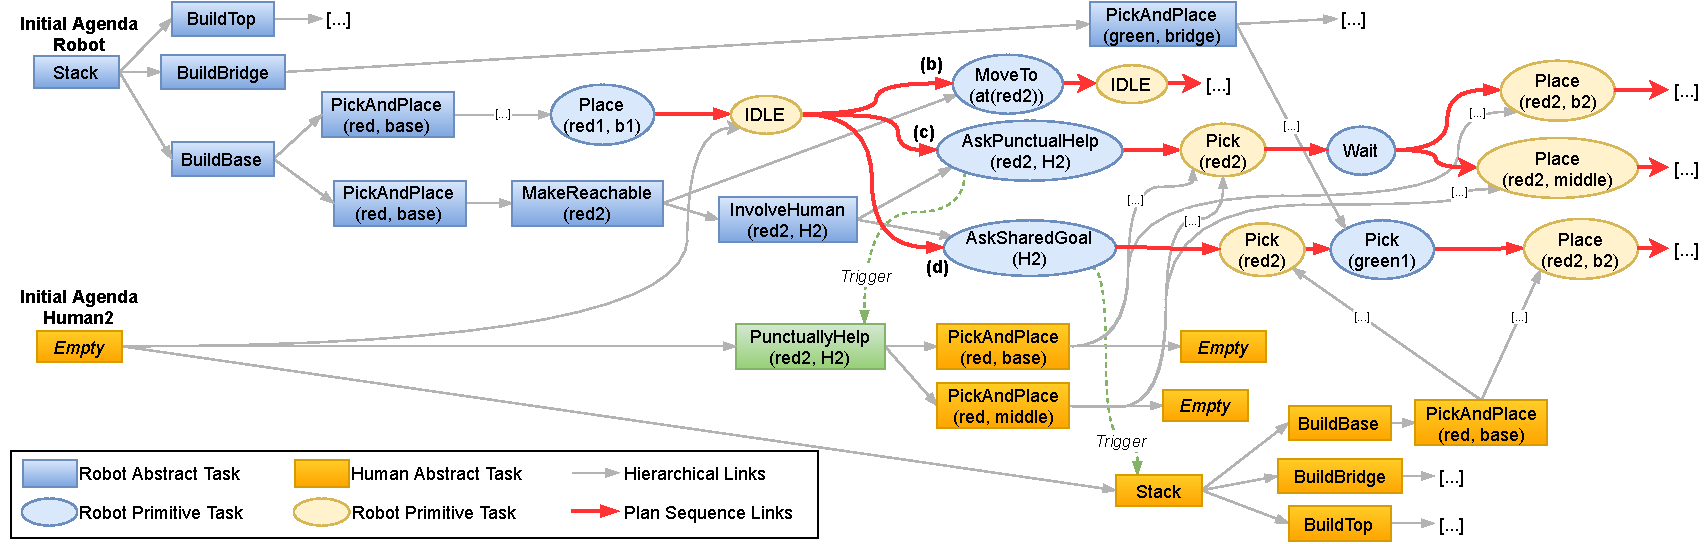
\includegraphics[width=0.65\linewidth]{Chapter3/plans.pdf}
    \caption{
    Plan obtained for the cooking scenario. 3 branches. Left: The human starts by adding salt. The only false belief is about \textit{``counterClean''}, which is irrelevant to the human agent. Hence, no communication is added. Middle: While the human is away, the robot turns on the stove and adds salt, creating two false beliefs. 
    Once back, we estimate that the human agent
    will be able to assess the observable fact \textit{``stoveOn''} but not \textit{``saltIn''}. Since the human agent might add salt again due to this false belief, it is relevant and fixed with a communication action. Right: The relevant false belief about \textit{``saltIn''} is avoided by delaying the robot's action until the human is co-present.
    }
    \label{fig:cooking_plan}
\end{figure}

Considering the cooking domain, we discuss in detail the plans obtained with our approach to a problem corresponding to the description given in the introduction. 
That is, there is no initial human false belief, agents both start in the kitchen, the pasta is in the adjacent room, the stove is off, and there is no salt in the water. The resulting plans are shown in Fig.~\ref{fig:cooking_plan}, and their detailed presentation explains how the approach works in practice. 
Since the human is uncontrollable and has different possible actions, the plan branches and the robot's actions differ in each case. 

In (\textit{left}), the human first adds salt, and then the robot turns on the stove. In both cases, thanks to the inference process, we estimate that the human will be aware of both facts about the salt (\textit{acting}) and the stove (\textit{co-present}). Then, while the human is away to fetch the pasta, the robot cleans the counter. Since the human is not co-present, their beliefs are not updated and now contain a false belief about the counter state. Once back, since \textit{counterClean} is not \textit{observable}, the observation process does nothing, and the false belief remains. However, this false belief does not affect human actions (non-relevant). Hence, there is no need to align human beliefs.

In (\textit{middle} and \textit{right}), the human begins by leaving the kitchen to fetch the pasta. First, let's focus on the (\textit{middle}) trace. The robot turns on the stove and adds salt while the human is away, creating two false beliefs. When returning to the kitchen, the observation process updates the human beliefs with the observable facts located in the kitchen. This fixes the false belief about \textit{stoveOn}. The robot then cleans the counter, which the human observes. 
However, without communication, the human's next action will be either ``add salt'' or ``ask the robot'', but considering the ground truth, the human could directly pour the pasta. Hence, the false belief on \textit{saltIn} is relevant and has to be corrected. Therefore, a communication is inserted in the robot's plan, and a ``delay'' branch is created (\textit{right}). 
In this delaying branch, the robot delays the add salt action until the human is co-present in order to make it observed (inference process) by the agent. 
In addition to this implicit communication, like in (\textit{middle}), the human assesses that the stove is on and can directly pour the pasta. 
\begin{table}[t]
    \centering
    \vspace{0.1cm}
    \caption
    {
    Success and communication ratio of different approaches. 
    }
    \label{tab:q_results}
    \begin{tabular}{@{}c|c c|| c| c@{}}
    % \begin{tabular}{c|c c|| c}
        \multirow{2}{*}{\textbf{Domain}} & \multicolumn{2}{c||}{\textbf{HATP/EHDA}} & \multicolumn{1}{c|}{\textbf{Only Comm}} & \multicolumn{1}{c}{\textbf{With Delay}}
        \\
        & \multicolumn{1}{c}{\textit{S}} & \multicolumn{1}{c||}{\textit{S I.Div.B.}} & \multicolumn{1}{c|}{\textit{Comm}} & \multicolumn{1}{c}{\textit{Comm}} 
        \\ \cline{1-5}
        \textit{Cooking}    &   18.6\%  &  6.9\%    & 69.5\% & 65.2\%\\
        \textit{Box}        &   25.0\%  & 14.3\%    & 79.7\% & 75.0\%\\
        \textit{Car}        &   12.5\%  & 0.0\%     & 68.8\% & 64.1\%\\
        \hline
        \textbf{Average}    &   18.7\%  & 7.1\%     & 72.6\% & 68.1\%\\
    \end{tabular}
\end{table}

\subsection{Experimental Results and Analysis}

In each domain, the actions and tasks remain the same. So here, a problem is defined by a starting agent ($R$ or $H$) and a pair of initial beliefs ($val^R_0, val^H_ 0$).
Initial ground truth ($val_0 \Leftrightarrow val^R_0$) is defined by setting each state-variable to an initial value. Five selected state-variables can have two possible values instead of one. Among these selected ones, three can diverge in human beliefs. These combinations generate 256 pairs of initial beliefs, where 12.5\% of them include initially aligned beliefs. Then, considering the starting agent, we obtain 512 problems for each domain. 
Each of the 1536 generated problems has been solved by HATP/EHDA, by \textit{our approach} using first \textit{only communication} and then using also \textit{delay}.
The obtained quantitative results appear in Table~\ref{tab:q_results}.
 
The overall success rate ($S$) and the one for initially diverging beliefs ($S I.Div.B.$) are shown for the HATP/EHDA solver. As expected, this solver always finds legal plans when dealing with initially aligned beliefs, and the low value of $S I.Div.B.$ reflects how poorly it handles belief divergences without specifically designed action models.
Our approach always finds legal plans, so we omitted its success rates in the last two columns, and we can say that it solves a broader class of problems.

Furthermore, considering the initially diverging beliefs and the divergences created along the planning process, more than $87.5\%$ of all problems involve belief divergences. 
However, only $72.6\%$ of the generated plans include communication actions when using only verbal communication.
This means that \textit{our approach} communicates only when necessary and not systematically. 
The amount of communication is even reduced to $68.1\%$ when delaying actions. In the latter case, only delayed branches that do not imply the human to wait are kept. 

%%% SECTION %%%%%%%%%%%%%%%%%%%%%%%%%%%%%%%%%%%%%%%%%%%%%%%%%%%%
\section{Discussion and Limitations}

This contribution has a few limitations to discuss.

First, the observability types of the state-variables are assumed to be constant. 
However, dynamic observability types permit modeling scenarios like an agent placing an object in an opaque box. The object would no longer be observable despite being in the same place as the agent. Since \textit{Places} can be symbolic, with clever domain modeling, one can model objects' disappearance when placed in a drawer. Dynamic observability types would simplify such modeling and make it even more expressive. However, this extension requires further research to correctly redefine Equation~\ref{eq:obs_update}. 

The underlying scheme allows just a single agent to execute a \textit{``real''} action at a time. 
However, a post-process can allow the execution of actions concurrently~\cite{CrosbyJR14}, however, note that the domain modeler has modeled $\mathcal{P}_{rh}$ as a sequential joint task. 
Parallelism is not considered in the current modeling and planning process, which limits the potential for concurrent executions.

We believe our modeling-level \acrshort{sa} proposals could fit in any other planning approach framing multi-party systems having one controllable agent while can only hypothesize remaining agents' behaviors (\textit{e.g.}, human-centered AI).

Agents' \acrshort{sa} models cannot simply refute a false belief, they can only assess new true facts to correct them.
For instance, assume the human \textit{wrongly} believes that the pasta is in \textsf{kitchen}. The \acrshort{sa} does not help refute this when the agent is in \textsf{kitchen}
because the state-variable \textit{NotAt(Pasta)} in \textsf{kitchen} is not modeled in our domain.  
However, such issues do not affect the completeness and, if necessary, our approach \textit{tackles} such cases as relevant false beliefs.

The relevance of estimated false human beliefs is challenging to determine. Currently, as soon as a divergence influences the next human actions, we assume that the divergence is likely detrimental to the goal and, thus, is relevant to be fixed. However, it would be interesting to find a method to evaluate the consequences of a divergence on the goal and plans in a principled way.

We discussed earlier that \acrshort{del} knowledge representation is more expressive, flexible, and can handle uncertainty. However, it requires an augmented action schema to accurately maintain each agent's beliefs.
Think of a specification for \textit{``move''} action manually listing all the environmental facts to be observed by an agent for managing their beliefs. In our case, it is implicitly maintained within a state.

We can consider running a set of rules (\textit{e.g.}, \textit{graph-based ontology}) to bring new interesting facts in the state based on a set of known facts. We believe that this aspect opens up new possibilities in the future for integrating human-aware collaborative planning and ontology.

%%% SECTION %%%%%%%%%%%%%%%%%%%%%%%%%%%%%%%%%%%%%%%%%%%%%%%%%%%%
% \section{Epistemic Extension}

% The planning process proposed in this contribution is part of the epistemic planning field. However, the uncertainties are limited and focused on the human decisions, in a simplistic manner compared to ``classical'' epistemic planner. Indeed, state-of-the-art epistemic planners consider epistemic states rather than ``simple'' beliefs and thus are able to keep track of several possible worlds. More precisely, [cite bolander] this work using the \acrshort{del} approach are able to keep track and reason on several possible worlds for each agent, and can even manage distinguishable worlds from others. Hence, the planner is able to anticipate that an agent can believe in three different possible worlds and tell that at execution time the agent will be able to distinguish if they are in world 1 or not, but they will not be able to tell distinguish between world 2 and 3 (based on observable facts).
% Such approaches currently heavily rely on conditional action effects and scripting. That is, when an agent enters a room with an action \textit{move}, the \textit{move} conditional effects will update accordingly the agent's possible worlds (the agent sees a box, notice that someone is not in the room anymore, and so on...). These situation assessment rules must be encoded into the action model used, and more precisely, in the action's effect which is not convenient and is domain specific.
% Our contribution proposes generalized situation assessment rules to maintain the beliefs but at the price to have simplified epistemic states.

% In some preliminary work we explored an extension of our approach to handle such classical epistemic representation. 

% * Describe first findings and models * 

% * Some results ? *

% * Discuss limitations: the current design is computationally very expensive and does not scale. Work on this aspect are needed and in progress to continue investigating this extension * 


%%% SECTION %%%%%%%%%%%%%%%%%%%%%%%%%%%%%%%%%%%%%%%%%%%%%%%%%%%%
\section{Conclusion}

This contribution is an extension of the HATP/EHDA human-aware task planner. 
The planner plans and implicitly coordinates the robot's actions with all estimated possible human (uncontrollable) behaviors that are then emulated to generate a new state.
Our extension and contribution are, first, to integrate a \textit{Situation Assessment} based reasoning system in the planner. This allows for maintaining distinct agents' beliefs based on what they can/should observe.
Compared to existing epistemic planners, this simplifies the action descriptions by focusing on their effects on the world and not how they influence each agent's beliefs.
In addition, we propose to detect false human beliefs and tackle only the necessary ones in a principled way. First, we propose minimal and proactive explicit communication. Second, when pertinent, 
we propose an implicit communication by postponing the non-observed robot action until the human is co-present to observe it.  
The relevance of false belief, when to optimally communicate, and parallelization are interesting future works.